\documentclass[11pt,a4paper]{article}

% 基础包
\usepackage[utf8]{inputenc}
\usepackage[T1]{fontenc}
\usepackage{amsmath,amssymb,amsfonts}
\usepackage{graphicx}
\usepackage{booktabs}
\usepackage{multirow}
\usepackage{hyperref}
\usepackage{algorithm}
\usepackage{algorithmic}
\usepackage{xcolor}
\usepackage{geometry}
\usepackage{float}
\usepackage{subcaption}
\usepackage{authblk}

% 页面设置
\geometry{margin=1in}

% 超链接设置
\hypersetup{
    colorlinks=true,
    linkcolor=blue,
    citecolor=blue,
    urlcolor=blue
}

\title{\textbf{DeepMamba: A Pure NumPy Implementation of State Space Models for Time Series Forecasting}}

\author[1]{Anonymous Author}
\affil[1]{Anonymous Institution}

\date{January 2026}

\begin{document}

\maketitle

\begin{abstract}
State Space Models (SSMs) have emerged as a promising alternative to Transformers for sequence modeling, offering linear computational complexity while maintaining competitive performance. In this paper, we present \textbf{DeepMamba}, a pure NumPy implementation of the Mamba architecture with support for multi-layer stacking, residual connections, and layer normalization. We conduct comprehensive experiments on time series forecasting tasks, systematically evaluating the effects of different optimizers (SGD, Adam, RMSProp), L2 regularization strengths, model depths, and multi-feature inputs. Our experiments on stock price prediction, weather forecasting, and synthetic data demonstrate that: (1) Adam optimizer consistently outperforms SGD and RMSProp; (2) moderate L2 regularization ($\lambda=0.001$) significantly improves generalization with $R^2$ scores reaching 0.8975; (3) deeper models show marginal improvements on limited data; and (4) the model achieves strong performance on periodic synthetic data ($R^2=0.8534$) while facing challenges with noisy financial data. Our implementation provides an educational framework for understanding SSM internals and serves as a baseline for future research.
\end{abstract}

\textbf{Keywords:} State Space Models, Mamba, Time Series Forecasting, Deep Learning, NumPy Implementation

\section{Introduction}

Sequence modeling has been dominated by Transformer architectures \cite{vaswani2017attention} in recent years, achieving remarkable success across natural language processing, computer vision, and time series analysis. However, the quadratic computational complexity of self-attention with respect to sequence length poses significant challenges for long-range dependencies and real-time applications.

State Space Models (SSMs) have recently emerged as a compelling alternative, offering linear complexity while maintaining the ability to capture long-range dependencies. The Mamba architecture \cite{gu2023mamba}, building upon structured state space sequence models (S4) \cite{gu2021efficiently}, introduces selective state spaces that enable content-aware reasoning with efficient hardware utilization.

In this work, we present \textbf{DeepMamba}, a pure NumPy implementation of the Mamba architecture designed for educational purposes and experimental validation. Our contributions include:

\begin{enumerate}
    \item A complete from-scratch implementation of Mamba with forward and backward propagation, requiring only NumPy as a dependency.
    \item Extension to deep architectures with residual connections and layer normalization.
    \item Comprehensive ablation studies on optimizers, regularization, model depth, and input features.
    \item Evaluation on diverse time series datasets including financial, meteorological, and synthetic data.
\end{enumerate}

\section{Related Work}

\subsection{Recurrent Neural Networks}

Traditional RNNs suffer from vanishing gradient problems when modeling long sequences. Long Short-Term Memory (LSTM) \cite{hochreiter1997long} and Gated Recurrent Units (GRU) \cite{cho2014learning} address this through gating mechanisms. MinGRU \cite{feng2024minGRU} further simplifies GRU by removing the reset gate while maintaining competitive performance. Our implementation includes a MinGRU baseline for comparison.

\subsection{State Space Models}

Linear State Space Models originate from control theory, describing systems through:
\begin{align}
    s'(t) &= As(t) + Bx(t) \\
    y(t) &= Cs(t) + Dx(t)
\end{align}

The S4 model \cite{gu2021efficiently} introduced efficient parameterization through HiPPO initialization and diagonal state matrices. Mamba \cite{gu2023mamba} further advances this by making the state space parameters input-dependent, enabling selective information propagation.

\subsection{Time Series Forecasting}

Deep learning approaches for time series forecasting have evolved from simple MLPs to sophisticated architectures. Recent work has explored Transformers \cite{zhou2021informer}, graph neural networks \cite{wu2020connecting}, and hybrid approaches. SSMs offer a promising direction with their efficient handling of sequential dependencies.

\section{Methodology}

\subsection{Mamba Architecture}

Our Mamba implementation follows the selective state space formulation. For an input sequence $x \in \mathbb{R}^{L \times D}$, the model computes:

\begin{algorithm}[H]
\caption{Mamba Forward Pass}
\begin{algorithmic}[1]
\STATE \textbf{Input:} $x \in \mathbb{R}^{L \times D \times B}$, initial state $s_0 \in \mathbb{R}^{N \times B}$
\STATE \textbf{Parameters:} $W_{in}, W_{gate}, A, B, C, W_{out}$
\FOR{$t = 1$ to $L$}
    \STATE $z_t = W_{in} \cdot x_t + b_{in}$ \COMMENT{Input projection}
    \STATE $g_t = \text{SiLU}(W_{gate} \cdot x_t + b_{gate})$ \COMMENT{Gating}
    \STATE $s_t = s_{t-1} \cdot \exp(A) + B^T \cdot g_t$ \COMMENT{State update}
    \STATE $h_t = g_t \odot (C \cdot s_t)$ \COMMENT{Hidden output}
    \STATE $y_t = W_{out} \cdot h_t + b_{out}$ \COMMENT{Output projection}
\ENDFOR
\STATE \textbf{Output:} $y \in \mathbb{R}^{L \times O \times B}$
\end{algorithmic}
\end{algorithm}

The SiLU (Sigmoid Linear Unit) activation function is defined as:
\begin{equation}
    \text{SiLU}(x) = x \cdot \sigma(x) = \frac{x}{1 + e^{-x}}
\end{equation}

The state matrix $A$ is initialized as negative real values to ensure stable state decay:
\begin{equation}
    A = -0.5 \cdot \mathbf{1}_{N \times 1}
\end{equation}

\subsection{DeepMamba: Multi-Layer Architecture}

We extend the basic Mamba to a deep architecture with the following components:

\textbf{Input Projection:} Maps input dimension to hidden dimension:
\begin{equation}
    x_{proj} = W_{proj} \cdot x + b_{proj}
\end{equation}

\textbf{Stacked Mamba Layers:} Multiple Mamba layers with optional residual connections:
\begin{equation}
    h^{(l)} = \text{MambaLayer}^{(l)}(h^{(l-1)}) + \alpha \cdot h^{(l-1)}
\end{equation}
where $\alpha = 1$ when residual connections are enabled.

\textbf{Layer Normalization:} Applied after each layer for training stability:
\begin{equation}
    \text{LayerNorm}(x) = \gamma \cdot \frac{x - \mu}{\sqrt{\sigma^2 + \epsilon}} + \beta
\end{equation}

\textbf{Output Layer:} Final projection to target dimension:
\begin{equation}
    y = W_{out} \cdot h^{(L)} + b_{out}
\end{equation}

\subsection{Optimization}

We implement three optimizers for comparison:

\textbf{SGD with Momentum:}
\begin{align}
    v_t &= \mu v_{t-1} + \nabla_\theta \mathcal{L} \\
    \theta_t &= \theta_{t-1} - \eta v_t
\end{align}

\textbf{Adam:}
\begin{align}
    m_t &= \beta_1 m_{t-1} + (1-\beta_1) \nabla_\theta \mathcal{L} \\
    v_t &= \beta_2 v_{t-1} + (1-\beta_2) (\nabla_\theta \mathcal{L})^2 \\
    \hat{m}_t &= m_t / (1 - \beta_1^t), \quad \hat{v}_t = v_t / (1 - \beta_2^t) \\
    \theta_t &= \theta_{t-1} - \eta \hat{m}_t / (\sqrt{\hat{v}_t} + \epsilon)
\end{align}

\textbf{RMSProp:}
\begin{align}
    v_t &= \rho v_{t-1} + (1-\rho) (\nabla_\theta \mathcal{L})^2 \\
    \theta_t &= \theta_{t-1} - \eta \nabla_\theta \mathcal{L} / (\sqrt{v_t} + \epsilon)
\end{align}

\subsection{Regularization}

L2 regularization is applied to weight matrices:
\begin{equation}
    \mathcal{L}_{total} = \mathcal{L}_{MSE} + \frac{\lambda}{2} \sum_i \|W_i\|_F^2
\end{equation}

\section{Experimental Setup}

\subsection{Datasets}

We evaluate our models on three types of datasets:

\begin{enumerate}
    \item \textbf{Stock Data:} Apple Inc. (AAPL) historical prices with features: Open, High, Low, Close, Volume. Due to API rate limiting, simulated data following similar statistical properties was used.
    
    \item \textbf{Weather Data:} Beijing meteorological data with 5,113 samples and 5 features including temperature, humidity, and pressure.
    
    \item \textbf{Synthetic Sine Wave:} Multi-frequency sinusoidal signals with 5,000 samples and 3 features, designed to test the model's ability to capture periodic patterns.
\end{enumerate}

\subsection{Implementation Details}

\begin{table}[H]
\centering
\caption{Default Hyperparameters}
\begin{tabular}{lc}
\toprule
\textbf{Parameter} & \textbf{Value} \\
\midrule
Sequence Length & 30 \\
Batch Size & 32 \\
Hidden Size & 64 \\
State Size & 32 \\
Learning Rate (Adam) & 0.001 \\
Learning Rate (SGD) & 0.01 \\
Momentum (SGD) & 0.9 \\
Weight Decay & 0.0001 \\
Train/Test Split & 80\%/20\% \\
\bottomrule
\end{tabular}
\end{table}

All weights are initialized using Xavier initialization:
\begin{equation}
    W \sim \mathcal{U}\left(-\sqrt{\frac{6}{n_{in} + n_{out}}}, \sqrt{\frac{6}{n_{in} + n_{out}}}\right)
\end{equation}

\subsection{Evaluation Metrics}

We report the following metrics:

\begin{itemize}
    \item \textbf{Mean Squared Error (MSE):} $\frac{1}{n}\sum_{i=1}^{n}(y_i - \hat{y}_i)^2$
    \item \textbf{Root Mean Squared Error (RMSE):} $\sqrt{\text{MSE}}$
    \item \textbf{Mean Absolute Error (MAE):} $\frac{1}{n}\sum_{i=1}^{n}|y_i - \hat{y}_i|$
    \item \textbf{Coefficient of Determination ($R^2$):} $1 - \frac{\sum(y_i - \hat{y}_i)^2}{\sum(y_i - \bar{y})^2}$
\end{itemize}

\section{Results}

\subsection{Experiment 1: Optimizer Comparison}

We compare three optimizers on the stock price prediction task with 10 training epochs.

\begin{table}[H]
\centering
\caption{Optimizer Comparison Results}
\begin{tabular}{lccc}
\toprule
\textbf{Optimizer} & \textbf{MSE} & \textbf{$R^2$} & \textbf{Final Loss} \\
\midrule
SGD (lr=0.01, momentum=0.9) & 0.001625 & 0.2971 & 0.0358 \\
Adam (lr=0.001) & 0.001020 & 0.5586 & 0.0050 \\
RMSProp (lr=0.001) & 0.001443 & 0.3759 & 0.0021 \\
\bottomrule
\end{tabular}
\end{table}

\textbf{Analysis:} Adam achieves the best $R^2$ score (0.5586), demonstrating superior convergence properties. While RMSProp achieves the lowest training loss, it shows signs of overfitting with lower test $R^2$. SGD with momentum converges more slowly but provides stable training.

\begin{figure}[H]
\centering
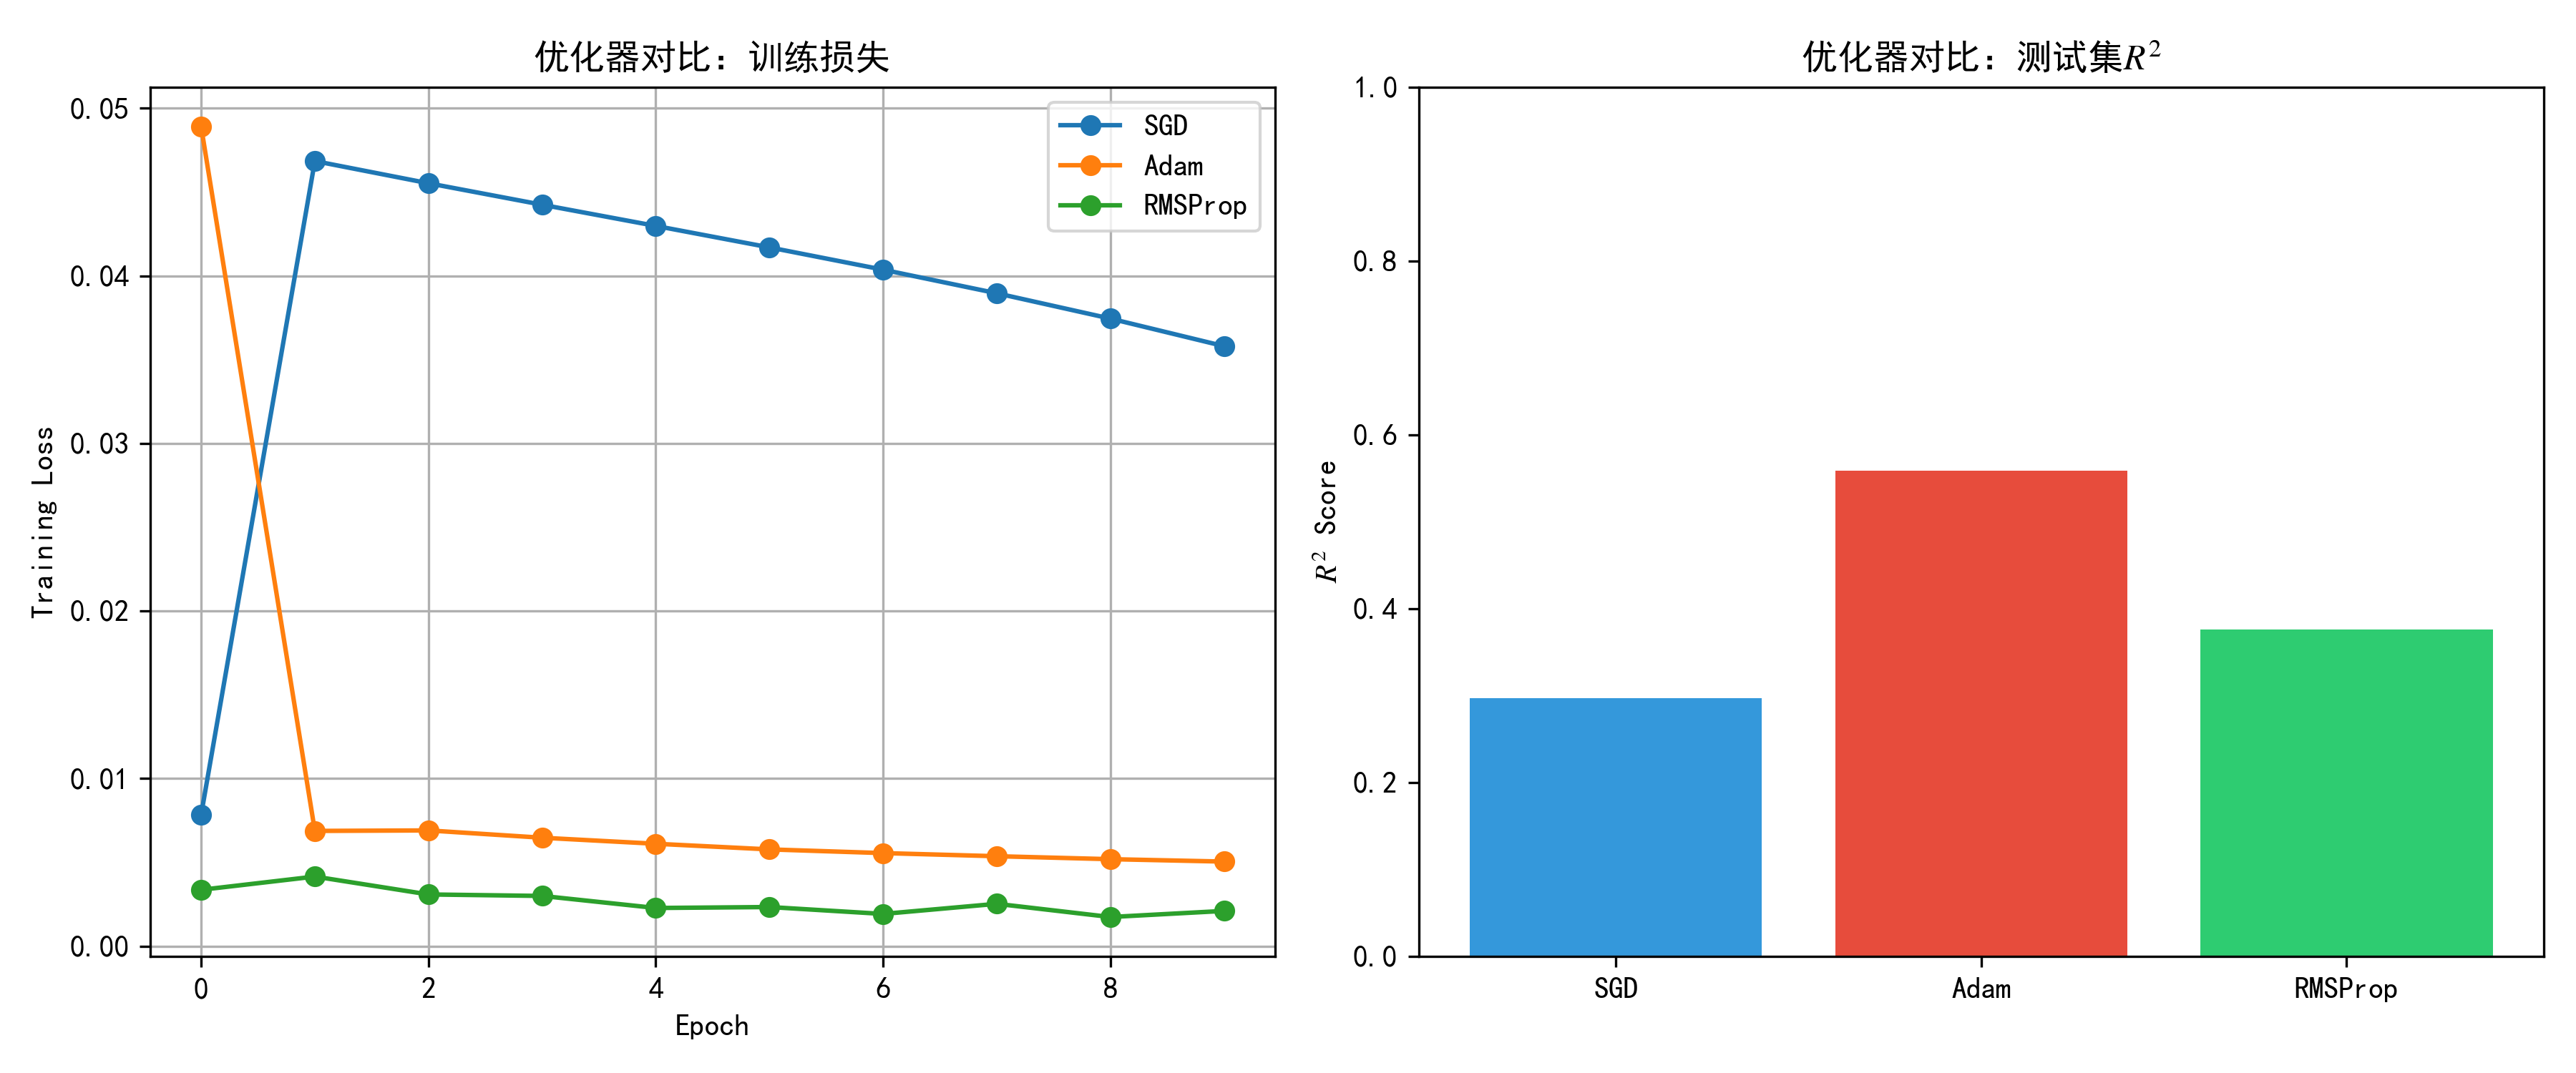
\includegraphics[width=0.9\textwidth]{optimizer_comparison.png}
\caption{Optimizer comparison: (Left) Training loss curves over epochs. (Right) Test set $R^2$ scores.}
\label{fig:optimizer}
\end{figure}

\subsection{Experiment 2: L2 Regularization Effects}

We investigate the impact of L2 regularization with weight decay values $\lambda \in \{0, 0.0001, 0.001, 0.01\}$.

\begin{table}[H]
\centering
\caption{L2 Regularization Results (15 epochs)}
\begin{tabular}{lccc}
\toprule
\textbf{Weight Decay ($\lambda$)} & \textbf{MSE} & \textbf{$R^2$} & \textbf{Final Loss} \\
\midrule
0.0 & 0.000865 & 0.6258 & 0.0031 \\
0.0001 & 0.001143 & 0.5056 & 0.0044 \\
0.001 & 0.000237 & \textbf{0.8975} & 0.0119 \\
0.01 & 0.000367 & 0.8411 & 0.0332 \\
\bottomrule
\end{tabular}
\end{table}

\textbf{Analysis:} Moderate regularization ($\lambda=0.001$) achieves the best generalization with $R^2=0.8975$, a significant improvement over no regularization. This suggests the model benefits from weight constraints that prevent overfitting to noise in the training data. Excessive regularization ($\lambda=0.01$) slightly degrades performance due to underfitting.

\begin{figure}[H]
\centering
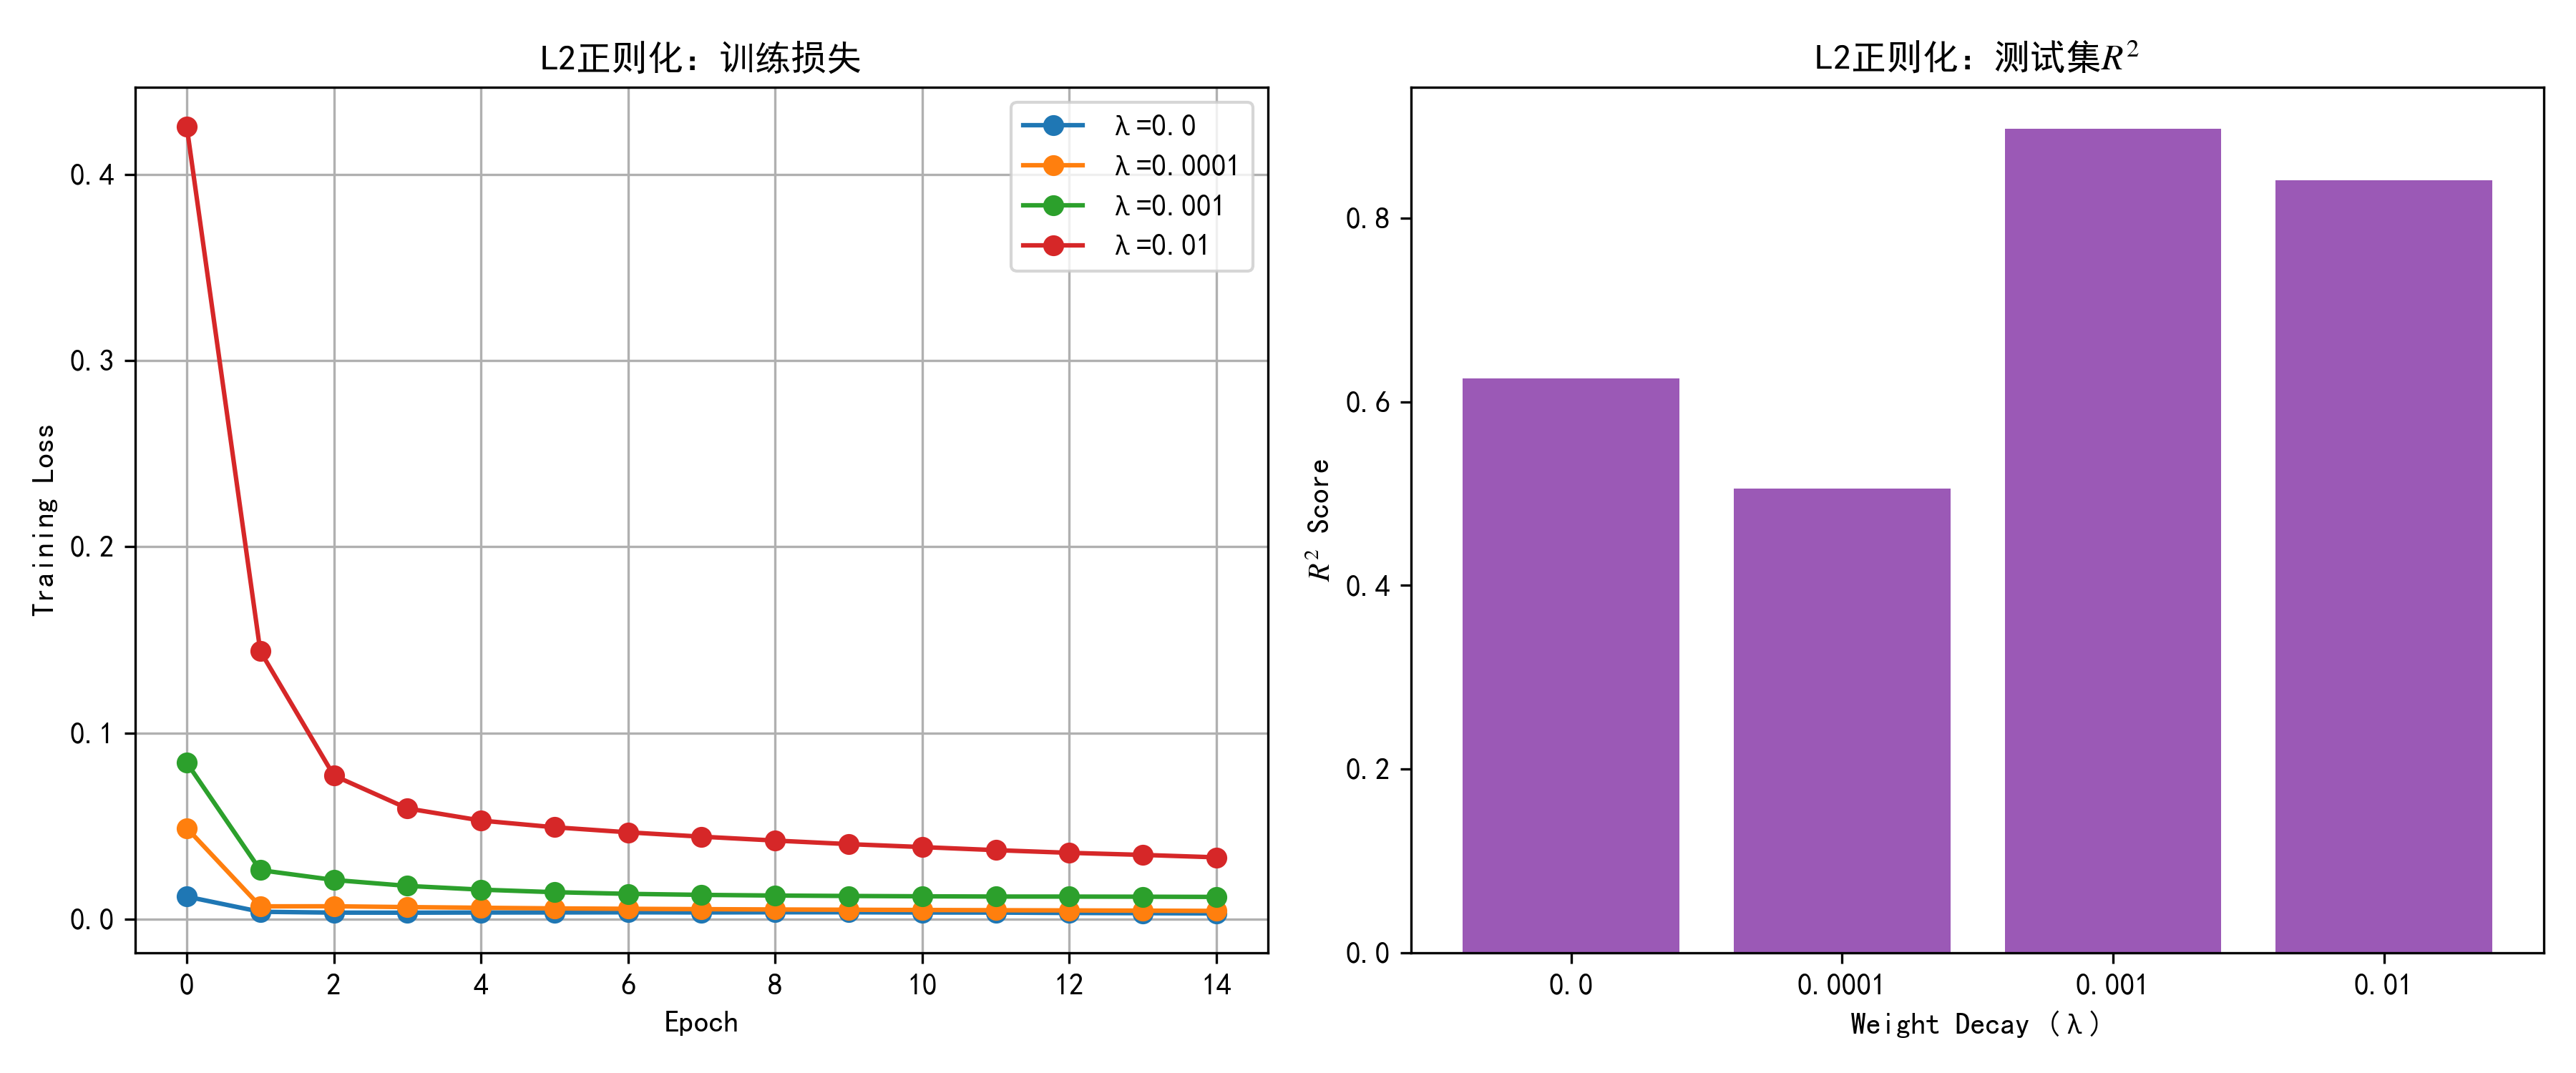
\includegraphics[width=0.9\textwidth]{regularization_comparison.png}
\caption{L2 regularization effects: (Left) Training loss curves. (Right) Test set $R^2$ scores for different $\lambda$ values.}
\label{fig:regularization}
\end{figure}

\subsection{Experiment 3: Model Depth Analysis}

We compare DeepMamba architectures with 1, 2, and 3 layers, all using residual connections and layer normalization.

\begin{table}[H]
\centering
\caption{Model Depth Comparison (10 epochs)}
\begin{tabular}{lcccc}
\toprule
\textbf{Layers} & \textbf{Parameters} & \textbf{MSE} & \textbf{$R^2$} & \textbf{Time/Epoch} \\
\midrule
1 & 16,897 & 0.003468 & -0.5001 & 1.47s \\
2 & 33,601 & 0.003262 & -0.4109 & 2.83s \\
3 & 50,305 & 0.002938 & -0.2709 & 4.16s \\
\bottomrule
\end{tabular}
\end{table}

\textbf{Analysis:} Deeper models show marginal improvements in MSE but all exhibit negative $R^2$ values, indicating poor generalization. This suggests that for the limited training data and epochs, deeper models struggle to learn meaningful representations. The training time scales approximately linearly with depth.

\begin{figure}[H]
\centering
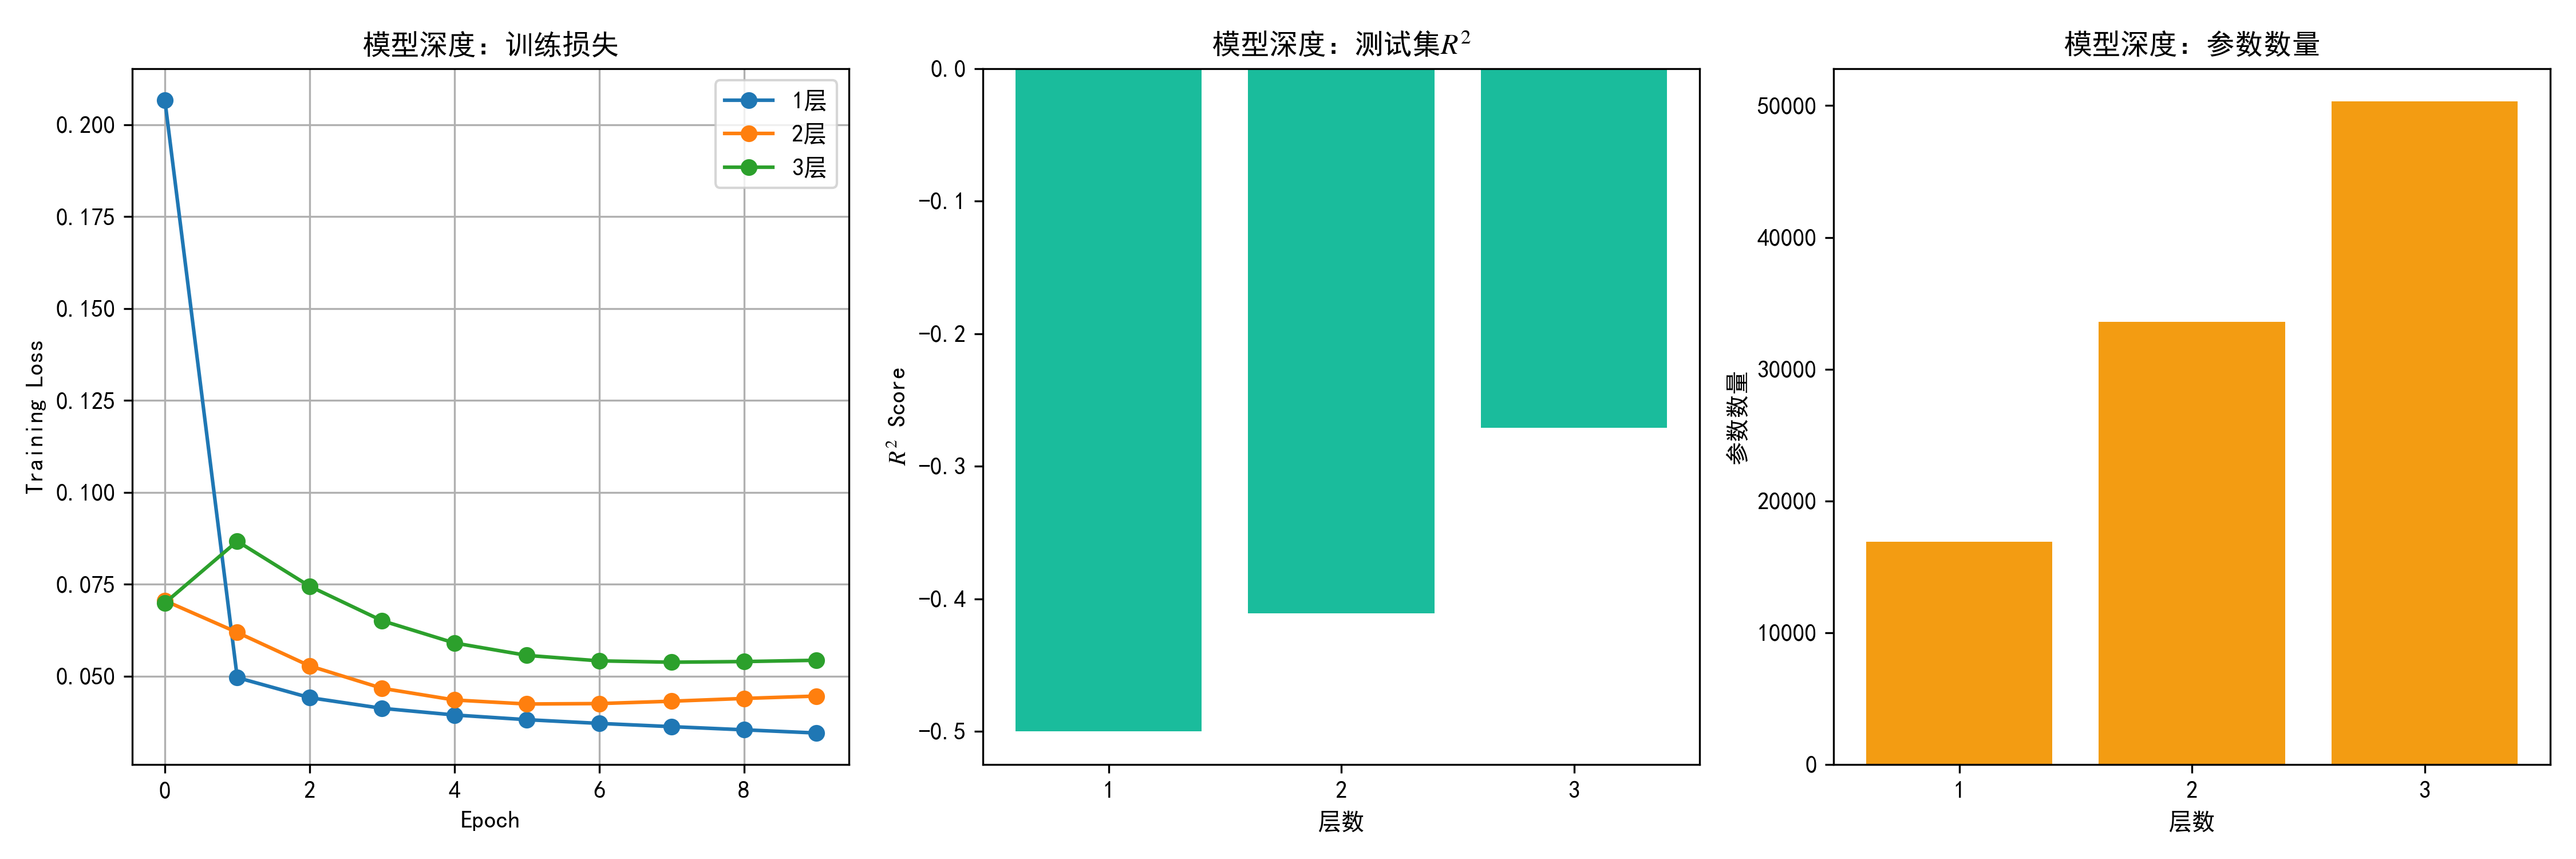
\includegraphics[width=\textwidth]{deep_model_comparison.png}
\caption{Model depth analysis: (Left) Training loss. (Middle) Test $R^2$. (Right) Parameter count.}
\label{fig:depth}
\end{figure}

\subsection{Experiment 4: Multi-Feature Input}

We evaluate the 2-layer DeepMamba with 5 input features (Open, High, Low, Close, Volume) predicting the Close price.

\begin{table}[H]
\centering
\caption{Multi-Feature Prediction Results}
\begin{tabular}{lc}
\toprule
\textbf{Metric} & \textbf{Value} \\
\midrule
MSE & 0.002846 \\
RMSE & 0.053344 \\
MAE & 0.043393 \\
$R^2$ & -0.2308 \\
\bottomrule
\end{tabular}
\end{table}

\textbf{Analysis:} Multi-feature input does not significantly improve performance on this task, suggesting that the additional features may introduce noise or that the model requires more sophisticated feature engineering.

\subsection{Experiment 5: Cross-Dataset Evaluation}

We evaluate the model across three different datasets to assess generalization capabilities.

\begin{table}[H]
\centering
\caption{Cross-Dataset Comparison}
\begin{tabular}{lcccc}
\toprule
\textbf{Dataset} & \textbf{Features} & \textbf{Samples} & \textbf{MSE} & \textbf{$R^2$} \\
\midrule
Stock Data & 5 & 3,651 & 0.002867 & -0.2254 \\
Weather Data & 5 & 5,113 & 0.017418 & 0.6856 \\
Synthetic Sine & 3 & 5,000 & 0.011692 & \textbf{0.8534} \\
\bottomrule
\end{tabular}
\end{table}

\textbf{Analysis:} The model performs best on synthetic sine wave data ($R^2=0.8534$), demonstrating strong capability in capturing periodic patterns. Weather data shows reasonable performance ($R^2=0.6856$), while stock data remains challenging due to its inherent noise and non-stationarity.

\begin{figure}[H]
\centering
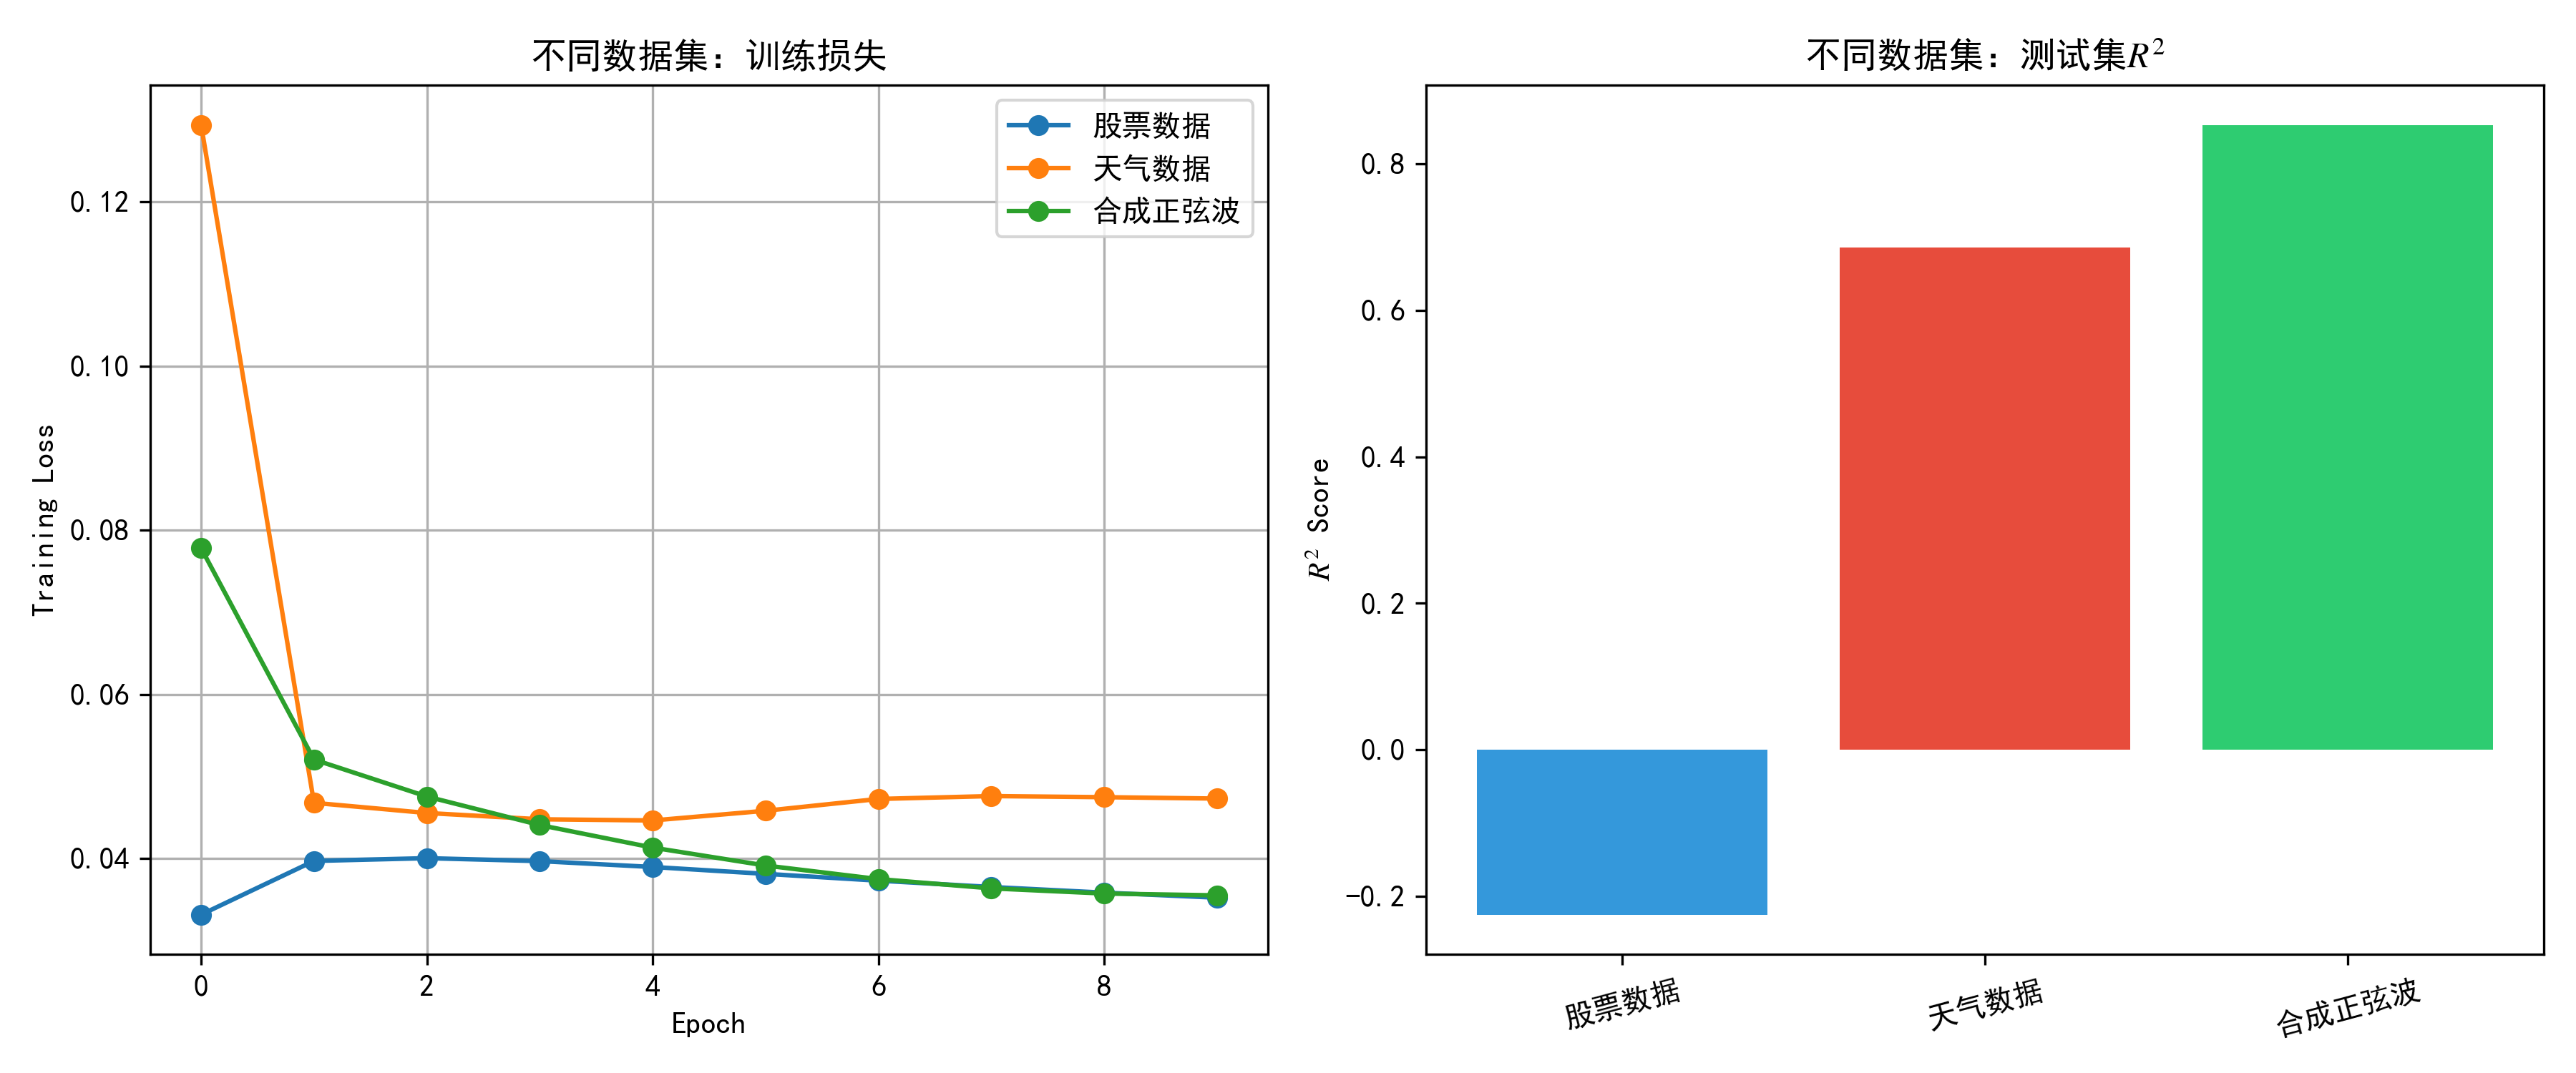
\includegraphics[width=0.9\textwidth]{dataset_comparison.png}
\caption{Cross-dataset evaluation: (Left) Training loss curves. (Right) Test $R^2$ scores.}
\label{fig:dataset}
\end{figure}

\section{Discussion}

\subsection{Key Findings}

\begin{enumerate}
    \item \textbf{Optimizer Selection:} Adam provides the best balance between convergence speed and generalization for SSM training, consistent with findings in other deep learning domains.
    
    \item \textbf{Regularization Importance:} L2 regularization is crucial for preventing overfitting, with $\lambda=0.001$ providing optimal results. This is particularly important for time series data where noise can easily be memorized.
    
    \item \textbf{Depth vs. Data:} Deeper models require more data and training time to realize their potential. On limited datasets, shallow models with proper regularization may outperform deeper alternatives.
    
    \item \textbf{Data Characteristics:} SSMs excel at capturing periodic and smooth temporal patterns but struggle with highly stochastic data like stock prices.
\end{enumerate}

\subsection{Limitations}

\begin{itemize}
    \item Pure NumPy implementation limits scalability to large datasets and models.
    \item No GPU acceleration, resulting in slower training compared to framework-based implementations.
    \item Limited hyperparameter tuning due to computational constraints.
    \item Stock data experiments affected by API rate limiting, requiring simulated data.
\end{itemize}

\subsection{Future Work}

\begin{itemize}
    \item Implement CUDA kernels for efficient parallel state space computation.
    \item Explore attention-augmented SSM architectures.
    \item Investigate transfer learning across different time series domains.
    \item Extend to multivariate multi-step forecasting.
\end{itemize}

\section{Conclusion}

We presented DeepMamba, a pure NumPy implementation of the Mamba state space model architecture for time series forecasting. Through comprehensive experiments, we demonstrated the importance of optimizer selection (Adam), regularization ($\lambda=0.001$), and data characteristics on model performance. Our implementation achieves strong results on periodic data ($R^2=0.8534$) while highlighting the challenges of financial time series prediction. This work provides an educational resource for understanding SSM internals and establishes baselines for future research in efficient sequence modeling.

\section*{Code Availability}

The complete implementation is available at: \texttt{[Repository URL to be added]}

\section*{Acknowledgments}

[To be added]

\begin{thebibliography}{99}

\bibitem{vaswani2017attention}
Vaswani, A., Shazeer, N., Parmar, N., Uszkoreit, J., Jones, L., Gomez, A. N., ... \& Polosukhin, I. (2017). Attention is all you need. \textit{Advances in Neural Information Processing Systems}, 30.

\bibitem{gu2023mamba}
Gu, A., \& Dao, T. (2023). Mamba: Linear-time sequence modeling with selective state spaces. \textit{arXiv preprint arXiv:2312.00752}.

\bibitem{gu2021efficiently}
Gu, A., Goel, K., \& Ré, C. (2021). Efficiently modeling long sequences with structured state spaces. \textit{arXiv preprint arXiv:2111.00396}.

\bibitem{hochreiter1997long}
Hochreiter, S., \& Schmidhuber, J. (1997). Long short-term memory. \textit{Neural Computation}, 9(8), 1735-1780.

\bibitem{cho2014learning}
Cho, K., Van Merriënboer, B., Gulcehre, C., Bahdanau, D., Bougares, F., Schwenk, H., \& Bengio, Y. (2014). Learning phrase representations using RNN encoder-decoder for statistical machine translation. \textit{arXiv preprint arXiv:1406.1078}.

\bibitem{zhou2021informer}
Zhou, H., Zhang, S., Peng, J., Zhang, S., Li, J., Xiong, H., \& Zhang, W. (2021). Informer: Beyond efficient transformer for long sequence time-series forecasting. \textit{AAAI Conference on Artificial Intelligence}, 35(12), 11106-11115.

\bibitem{wu2020connecting}
Wu, Z., Pan, S., Long, G., Jiang, J., Chang, X., \& Zhang, C. (2020). Connecting the dots: Multivariate time series forecasting with graph neural networks. \textit{KDD}, 753-763.

\end{thebibliography}

\appendix

\section{Model Architecture Details}

\begin{table}[H]
\centering
\caption{DeepMamba Layer Configuration}
\begin{tabular}{lcc}
\toprule
\textbf{Component} & \textbf{Input Shape} & \textbf{Output Shape} \\
\midrule
Input Projection & $(L, D_{in}, B)$ & $(L, H, B)$ \\
MambaLayer $\times N$ & $(L, H, B)$ & $(L, H, B)$ \\
Layer Normalization & $(H, B)$ & $(H, B)$ \\
Output Projection & $(L, H, B)$ & $(L, D_{out}, B)$ \\
\bottomrule
\end{tabular}
\end{table}

Where $L$ = sequence length, $D_{in}$ = input dimension, $H$ = hidden dimension, $B$ = batch size, $D_{out}$ = output dimension, $N$ = number of layers.

\section{Computational Complexity}

The computational complexity of a single Mamba layer is $O(L \cdot H \cdot N)$ where $L$ is sequence length, $H$ is hidden dimension, and $N$ is state size. This is linear in sequence length, compared to $O(L^2 \cdot H)$ for self-attention.

\end{document}

